\documentclass[pdftex]{article}
\usepackage[pdftex]{graphics}
\usepackage{subfigure}
\usepackage{hhline}
\usepackage[usenames,dvipsnames]{color}
\usepackage{colortbl}
\usepackage[screen,pdftex]{mcdlecture}
\newcommand{\bs}{\relax}
\newcommand{\es}{\newpage}
\fboxsep=.01\textwidth \fboxrule=1pt
\newsavebox{\savepar}
\newenvironment{boxit}{\begin{lrbox}{\savepar}
    \begin{minipage}[b]{0.975\textwidth}}
    {\end{minipage}\end{lrbox}\framebox{\usebox{\savepar}}}


%%%%%%%%%%%%%%%%%%%%%%%%%%%%%%%%%%%%%%%%%%%%%%%%%%%%%%%%%%
%% THE FOLLOWING ARE THINGS THAT WE MIGHT CHANGE FROM YEAR TO YEAR OR
%% VENUE TO VENUE
    \lhead{MCMC in Statistical Genetics}
    \lfoot{Dr Eric C. Anderson and Dr Matthew Stephens}
%	\lfoot{Dr Eric C. Anderson and Dr John Novembre}
%    \rfoot{UW - Summer Institute, July 2013}
%	 \rfoot{Edinburgh - European Institute, June 2012}
\rfoot{Brazil - Summer Institute, February 2014}

% on this one, be sure to update the venue and the module number
%\newcommand{\coursetitlepage}{European Institute in Statistical Genetics
%\newcommand{\coursetitlepage}{Summer Institute in Statistical Genetics
\newcommand{\coursetitlepage}{Brazilian Edition of the Summer \\Institute in Statistical Genetics

Module 9:

MCMC for Genetics}

%% Then update the schedule.  Note that I have broken that
%% out into a separate file like: schedule_table_edinburgh2012.tex
%% which is input in Overview.tex

%% Then be sure to change any time-sensitive events in the 
%% probability discussion in Matthew's first lecture.

%% And also update "structure_fun" link to my wiki to the right
%% year and venue.
%%%%%%%%%%%%%%%%%%%%%%%%%%%%%%%%%%%%%%%%%%%%%%%%%%%%%%%%%%


\begin{document}

\DeclareGraphicsExtensions{.jpg,.pdf,.png}%



%% Eric added a few things:
% some commands that Eric made for making a title while starting
% a new lecture and for making titles of new slides.
\newcommand{\newlecture}[1]{\newpage\begin{center}\section*{#1}\end{center}}
\newcommand{\newslide}[1]{\newpage\subsection*{#1: \hfil}}
 \newcommand{\Exp}{\Bbb{E}}
 \newcommand{\Var}{{\mathrm{Var}}}
 %% Some pretty etc.'s, etc...
\newcommand{\cf}{{\em cf.}}
\newcommand{\eg}{{\em e.g.},}
\newcommand{\ie}{{\em i.e.},}
\newcommand{\etal}{{\em et al.}\ }
\newcommand{\etc}{{\em etc.}}

%% some handy things for making bold math
\def\bm#1{\mathpalette\bmstyle{#1}}
\def\bmstyle#1#2{\mbox{\boldmath$#1#2$}}
\newcommand{\thh}{^\mathrm{th}}
\newcommand{\bpi}{{\pi}}
\newcommand{\mP}{\mathbf{P}}

\rhead{Session 6 - \thepage}
 
\newcommand{\bY}{{\bm{Y}}}
\newcommand{\bX}{{\bm{X}}}

 
\newlecture{Computing Practical Session \\ with {\em structure}}
The goals of this practical session---Allow students to:
\begin{itemize}
\item Familiarize themselves with {\em structure}'s data format
\item Use the {\em structure} front end
\item Understand how the structure front end prepares input files 
\item Analyze the Scottish cats data
\item Examine the output from {\em structure} to gain familiarity with visually assessing
convergence of different MCMC chains.
\end{itemize}

\newslide{Structure data format}
\begin{itemize}
\item {\em structure} expects data in white-space delimited rows
\item The genotypes of individuals can be recorded in a single row, or
in multiple rows.  The cat data uses a single row for each individual.
\item The first row holds the marker names (\eg{} ``fca8 fca23 \ldots").
\item Each individual's row contains the individual's ID (in the first column---\eg{} ``Z12"), then an integer specifying its population or sampling location information (in the second column---\eg{} ``3").  The remaining columns are the genotypes (two columns for each locus, \eg{} ``123 143 \ldots").
\item These are {\em microsatellite} genotypes.  Each diploid individual has two gene copies, and the different alleles are different lengths of simple repeat DNA segments between conserved primer regions.  
\item Such data are not used extensively in human genetics any longer, but are still used in molecular ecology.  In this case they provide a compact data set that {\em structure} can analyze quickly enough to do multiple runs in the course of a short practical session.
\item The first five lines of {\sl cats.dat} are below:
\end{itemize} 
{\footnotesize
\begin{verbatim}
fca8      fca23  fca35  fca43  fca45  fca77  fca90  fca96  fca126
Z12 3   123 143 136 140 144 144 120 122 157 158 144 144 107 107 210 212 142 144
Z13 3   135 135 134 140 144 144 120 122 161 161 144 144 93  105 210 220 144 144
Z14 3   115 121 132 150 144 152 118 122 152 158 144 144 107 113 214 220 142 142
Z15 3   121 123 140 140 144 152 122 128 152 152 144 144 93  107 212 210 136 142
\end{verbatim}
}
$\bullet$ Sampling localities 1--6 refer to wild-living cats in Scotland, and localities 7, 8, and 9 refer to house cats sampled from veterinary centers in three regions in the southern UK.



\newslide{Making a new {\em structure} project file}
\begin{itemize}
\item The Java-based front end of {\em structure} organizes MCMC runs in the form of projects.  
\item Each run in a project uses the same data set, but can use different parameter settings for different runs.  
\item The front end accomplishes this by preparing appropriate input files for {\em structure} then issuing the appropriate commands to run structure with those input files. It is convenient for people who are not very comfortable in a command line environment.  
\item The front end also has some useful data visualization capabilities.  
\item To make a new {\em structure} project to analyze the {\em cats.dat} data set:
\begin{enumerate}
\item Launch {\em structure} (usually by double-clicking its icon or its shortcut).  This launches the front end.
\item Go back to {\em structure} and choose [File]$\rightarrow$[New Project\ldots] to launch the ``Project Wizard".  Then give the project a name (I would recommend not putting spaces in the name).  In the rest of this, we will assume we have named the project ``scot-cats".  Select the directory you wish to put it in (I just put it on my Desktop) and then select the data file {\sl cats.dat} which is part of the SISG module's data.  Or, if you wish to download it directly, you can get it from \url{http://tinyurl.com/scot-cats}.  Once you download it, you have to direct {\em structure} to where the file resides in your file system.
\begin{center}
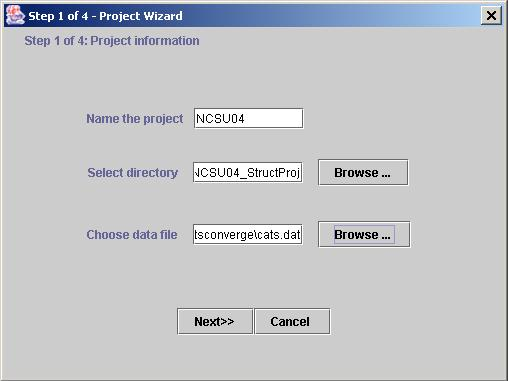
\includegraphics[width=.56\textwidth]{illus/projsetup.jpg}
\end{center}
\item In Step~2 of the ``Wizard" we have to report how many individuals and loci there are in the files.  Choose ``Show data file format" to get a little information about the file:
\begin{center}
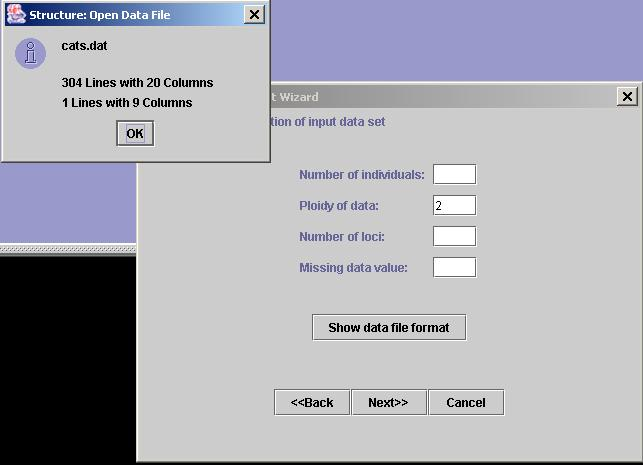
\includegraphics[width=.66\textwidth]{illus/dataformat.jpg}
\end{center}
One can see there is one row with 9 locus names then 304 rows of individuals, with 20 columns ($2 \times 9$~for the loci, plus one for the ID, and one for the population label).  So fill in these values:
\begin{itemize}
\item Number of individuals: 304
\item Ploidy of data: 2 
\item Number of loci: 9
\item Missing data value -9
\end{itemize}
(If you look through the file you see that missing data values are coded as -9's). Then hit next\ldots.
\item Step 3 of the ``Wizard":  More data file formatting setup.  Check the boxes for ``Row of marker names" (because the file starts with a row of locus names) and also for ``Data file stores data for individuals in a single line."
\begin{center}
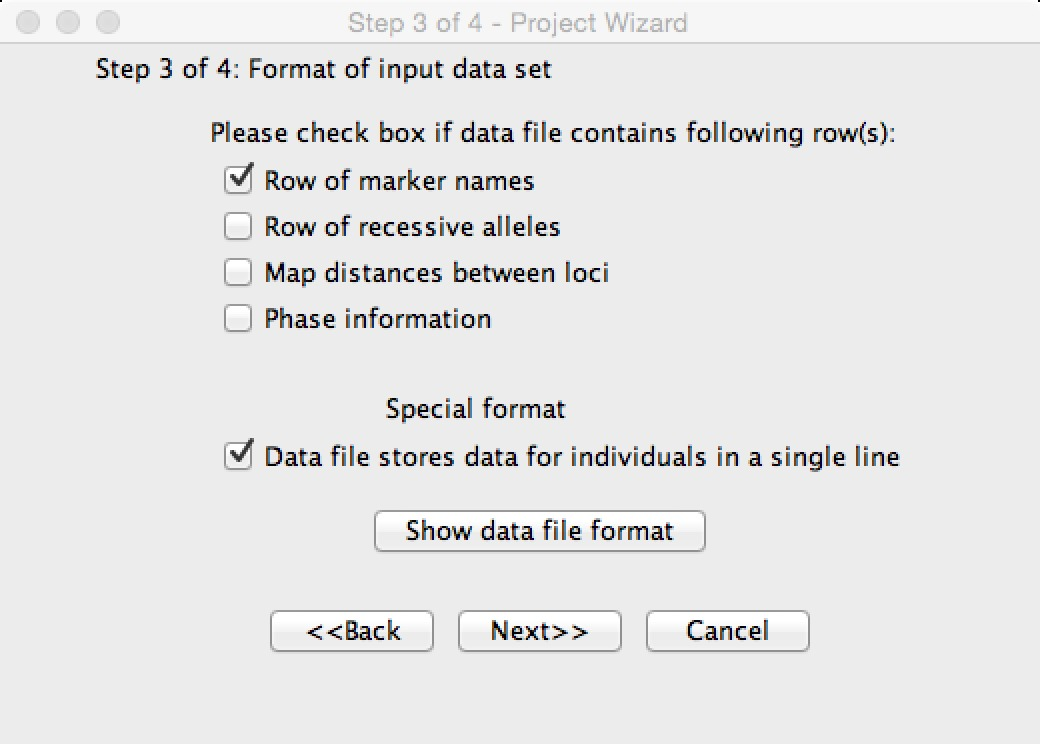
\includegraphics[width=.66\textwidth]{illus/dataformat2.jpg}
\end{center}
\item Step 4 of the ``Wizard": Here we have to alert {\em structure} to any other columns that exist for each individual in a row.  Recall that we have an ID for each indiv, and also an integer expressing sampling location.  So check the boxes next to ``Individual ID for each individual" and ``Putative population origin for each individual."  
\begin{center}
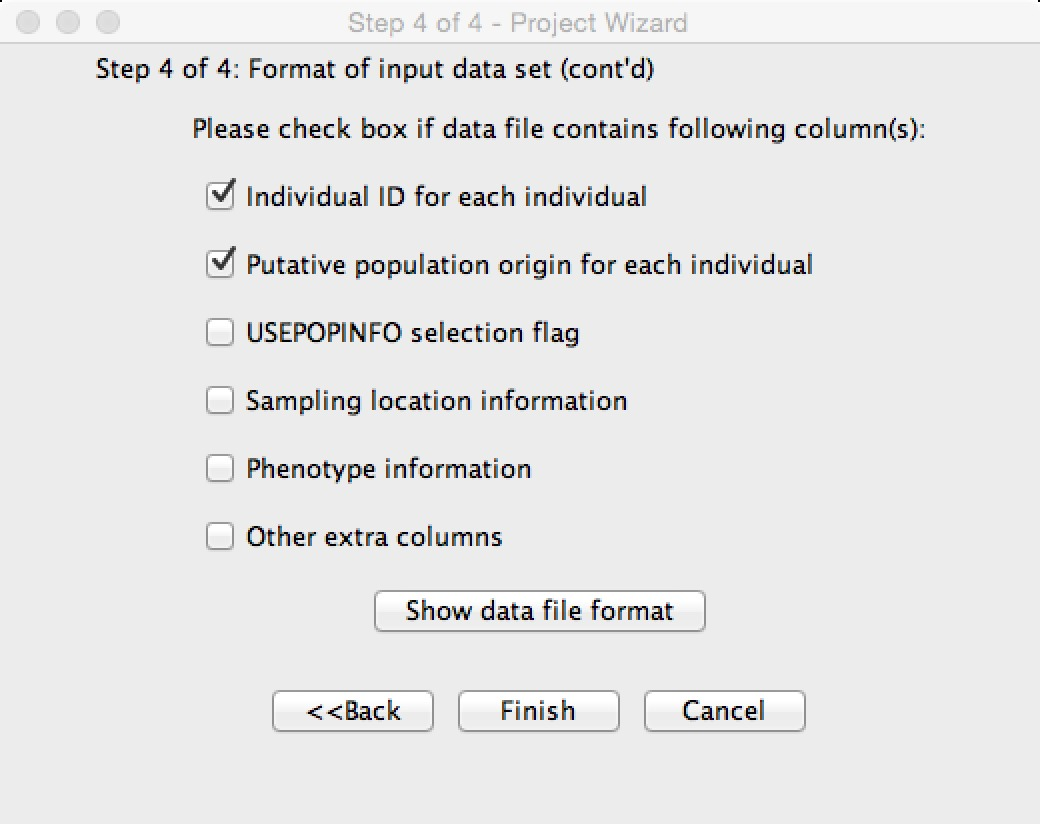
\includegraphics[width=.66\textwidth]{illus/dataformat3.jpg}
\end{center}
Then hit Finish.  Then Proceed.


\item That should work, and you should see the data in a spreadsheet window.  Now we must specify parameters for a run.
\end{enumerate} 
\end{itemize}

\newslide{Creating parameter sets}
\begin{enumerate}
\item Choose [Parameter Set]$\rightarrow$[New\ldots]
\item Note that there are tabs to set the Run Length, Ancestry Model, Allele Frequency Model, and ``Advanced" options.
\item Let's do a simple parameter set with mostly default options.  We want to get things done pretty quickly, so we will do shorter runs than are typically recommended.  Set Burn In at 2000 and MCMC reps after burn-in to 4000. 
\item We will use the admixture model with correlated frequencies, etc.  These are all the default options.
\item Hit OK, and then name the parameter set.  For this example I will name it ``PlainPars".  Hit OK.  You should now see a summary of the parameter set.
\item Try clicking around in the left hand panel to see the different views of data and parameter sets that are now available.  
\end{enumerate}

\newslide{Doing a {\em structure} run}
\begin{itemize}
\item We can now do a run of {\em structure} using the parameters in PlainPars.  Do this by choosing [Parameter Set]$\rightarrow$[Run]. Set the number of assumed populations ($K$) to 2 and hit OK.
\item While this is running, you can view traces of some of the important parameters.  For example, choose [Plotting]$\rightarrow$[Run-time]$\rightarrow$[Alpha] to view a trace of values of $\alpha$ inferred by {\em structure}.  
\item Be sure to kill the trace plot windows when you are done with them because (at least on older versions I used) they slow down the progress immensely.  
\item When the run has finished, click on ``Results" under ``PlainPars" in the left panel, so it expands out and you can click on ``PlainPars\_run\_1 (K=2)".  With that highlighted, the right panel should give the text summary of the {\em structure} output, and the right panel also has pull-down menus to plot the output in various ways:
\end{itemize}
\begin{center}
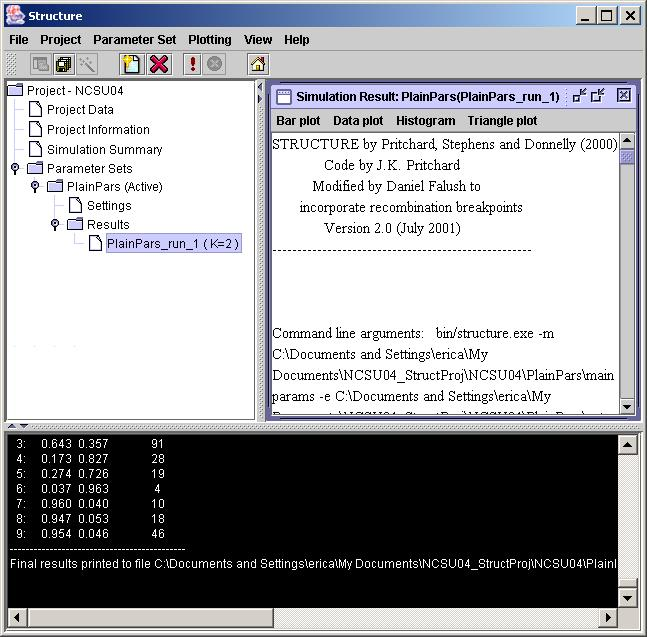
\includegraphics[width=.66\textwidth]{illus/Run1.jpg}
\end{center}


\newslide{Plotting results using the front end}
From the right hand window when results of any run are selected you can 
\begin{itemize}
\item Make a Bar Plot that shows each individual's $\bm{Q}$ (admixture proportions).  To get this plot, choose [Bar plot]$\rightarrow$[Show].  To see it up closer, you can select the ``Plot in multiple lines" radio button.  The result should look like:
\end{itemize}
\begin{center}
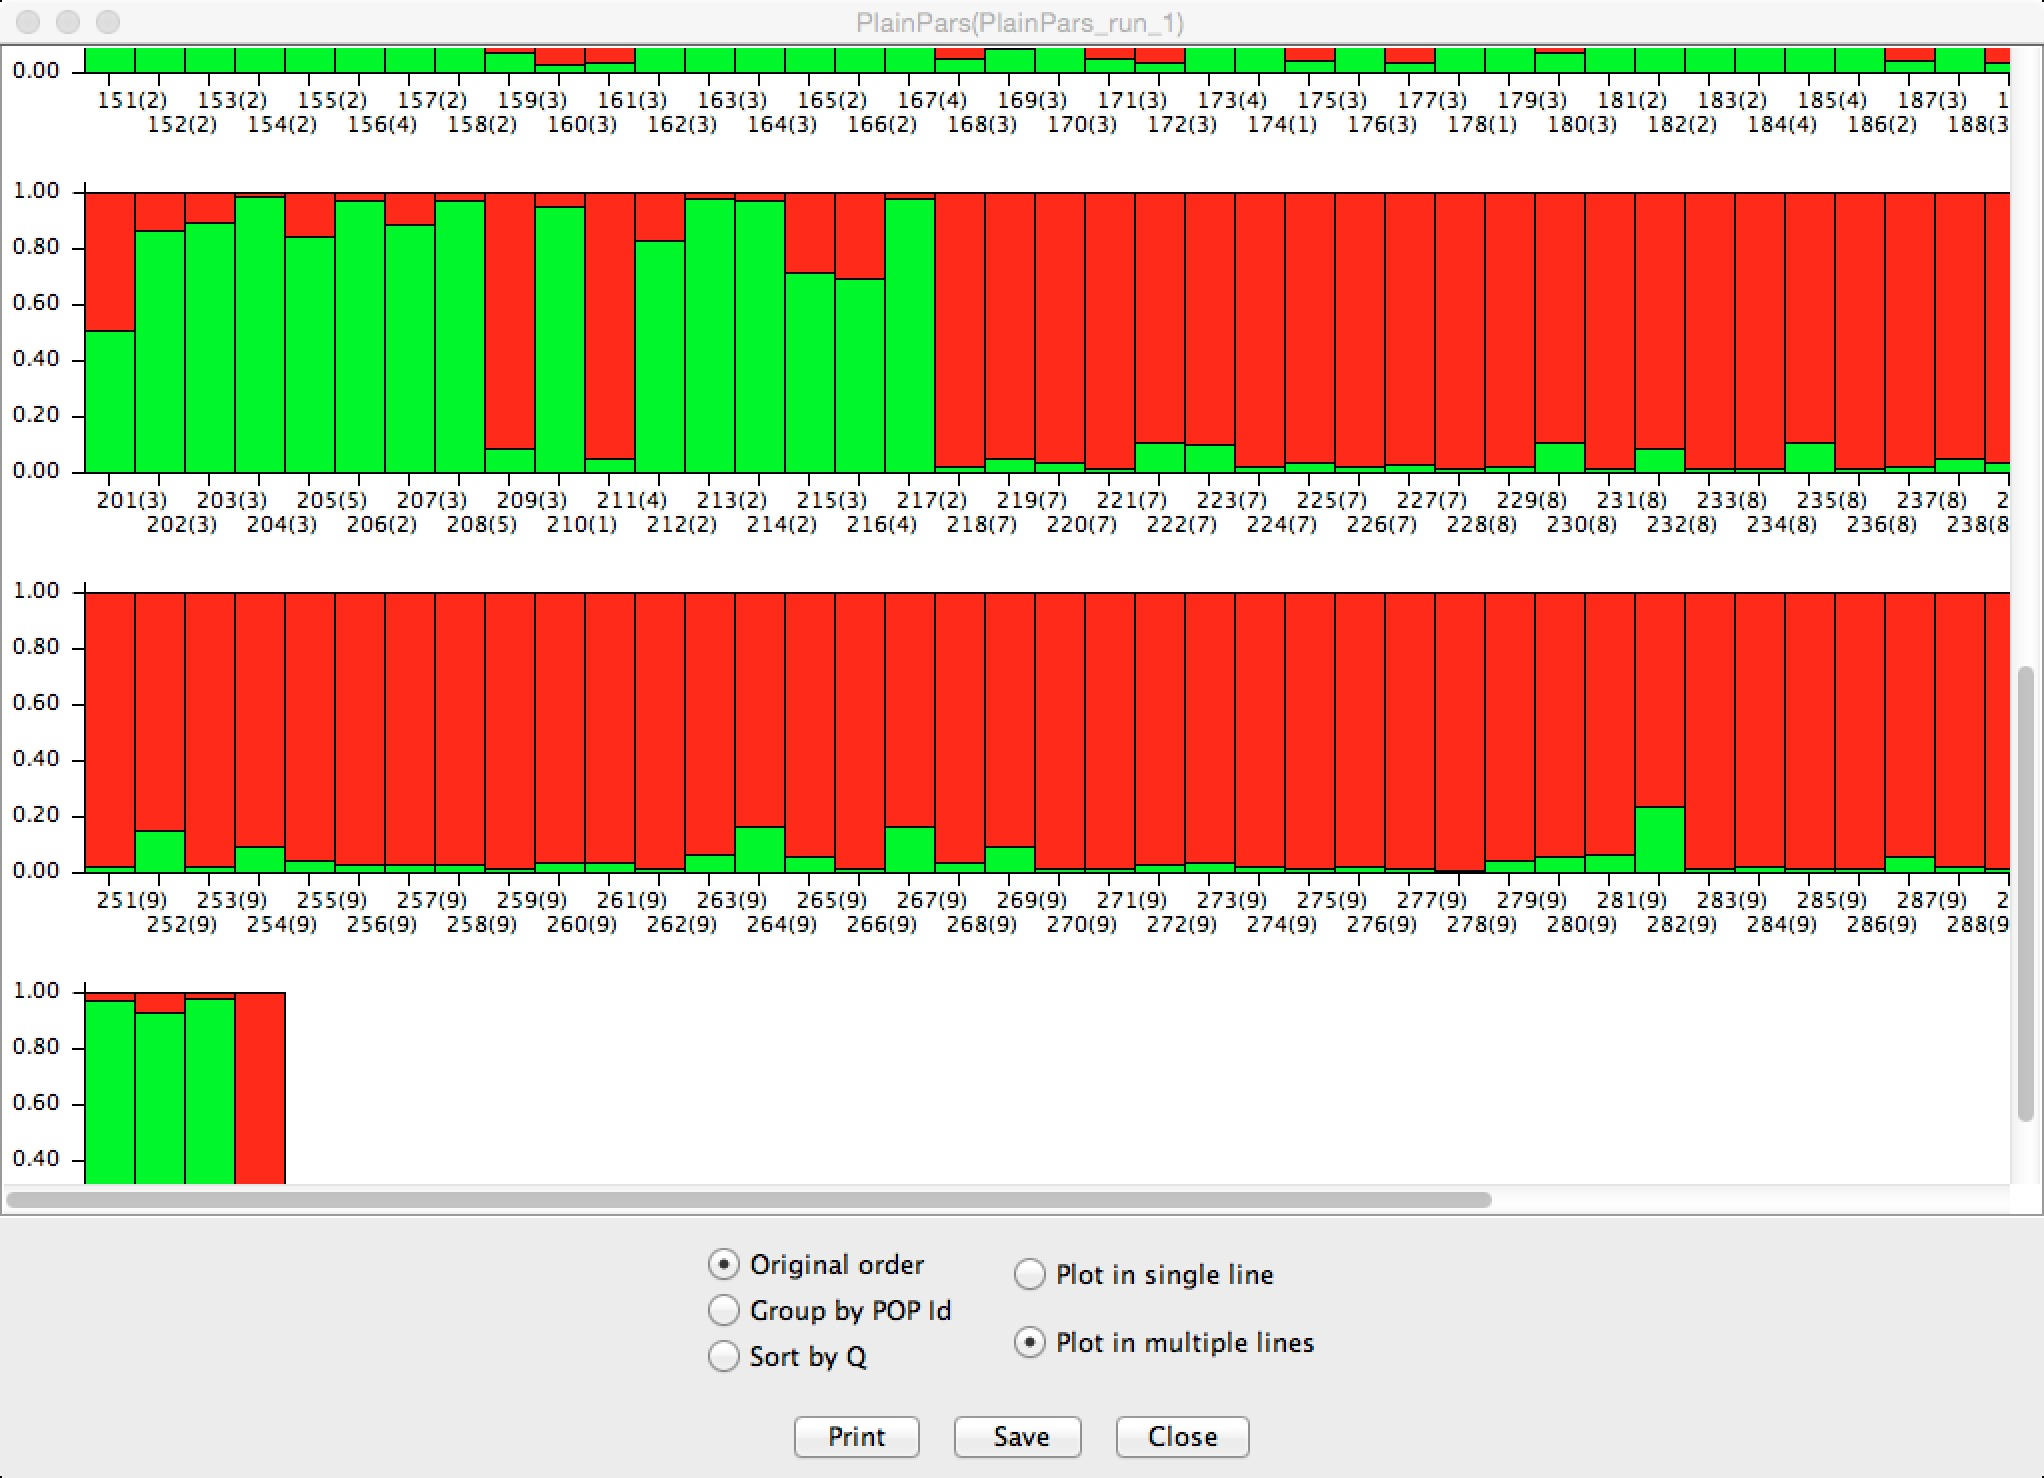
\includegraphics[width=.66\textwidth]{illus/barplot.jpg}
\end{center}
Scroll through this plot and note that the individuals from sampling locales 7, 8, and 9, (the house cats) consistently have a large proportion of ancestry from one of the subpopulations.  That subpopulation presumably represents domestic cat ancestry.  Interestingly, some of the wild-living cats have just as much ``domestic cat ancestry" as do the cats from the vet clinics.  

\begin{itemize}
\item You can also plot traces of variables like $\alpha$, and the complete data log likelihood.  Choose [Data plot] for these.  These can give you some idea of how well the MCMC is mixing.  
\item Try creating some histogram plots, as well.  
\end{itemize}

\newslide{The underlying parameter files}
When the front end executes a run of {\em structure}, it creates a {\sl mainparams} and an {\sl extraparams} file.  These are the files that you would use to execute the same run on the command line.  

To see what these files look like, you can find these two files in the PlainPars directory in your {\em structure} project folder, and open them up with any suitable text editor
\begin{center}
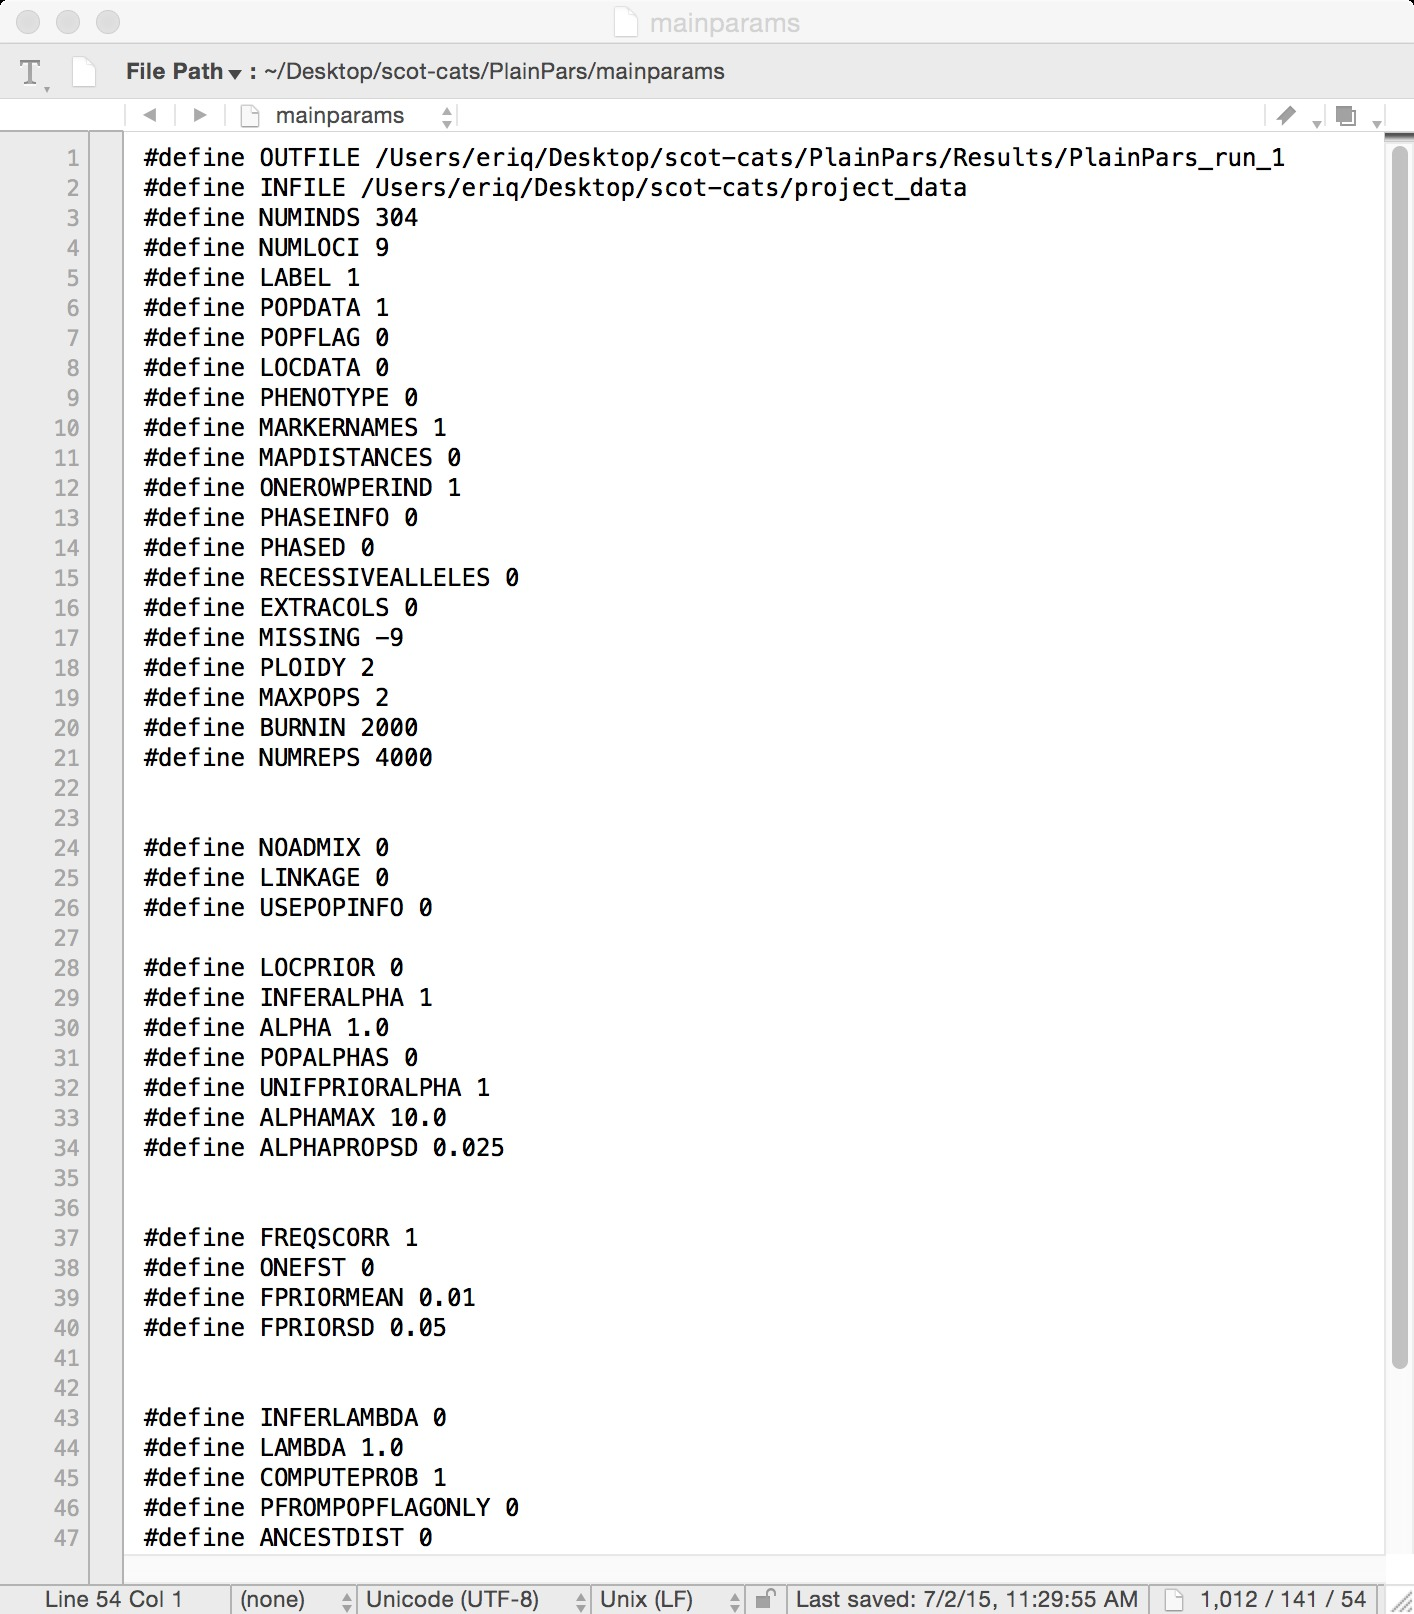
\includegraphics[width=.90\textheight]{illus/mainparams.jpg}
\end{center}
%There is a feature that allows you to generate these parameter files, without running them, but it seemed buggy on the version I have.  


\newslide{Scheduling a series of runs}
One very useful feature of the front end is that it allows you to set up a series of runs.  This is especially useful for investigating different values of $K$.  

We will use this feature to investigate model selection for different values of $K$:
\begin{enumerate}
\item Select [Project]$\rightarrow$[Start a Job]
\item Then select ``PlainPars" from the Structure Scheduler
\item Set K from 1 to 4
\item Set the number of iterations to 2 (or more if your computer crunches through each run
in little time.)
\item Hit start.  
\end{enumerate}

That should finish in a few minutes.  Once it is done, note that all the results are neatly stored in the Results directory of the left panel.  

If you did more than one iteration for each $K$, compare the values obtained for $\mathrm{Ln} P(D)$ in the different runs at the same value of $K$.  Especially for $K=4$ there may be marked disparities due to mixing anomalies.  

Look at trace plots of the Ln Likelihood values for runs that look like they may be a little anomalous.

Remember that inference for $K$ using {\em structure} is quite {\em ad hoc}. 

\newslide{Assessing Convergence By Examining Traces}
One of the unfortunate deficiencies of the {\em structure} front end is that it does not
print out all the standard output of the program structure.  That output includes current
values of a number of variables in the MCMC every sweep.  Instead, those data are stored
within Java objects by the {\em structure} front end.  

While that approach allows you to make trace plots for single runs in the front end, it is hard to compare the results from multiple runs.

Since one of the themes of this course is that it is essential to compare the results from
multiple MCMC chains, we've prepared a little R package that makes it easy to do multiple
runs of {\em structure} and then compare the runs using the R package {\tt ggplot2}.

\enlargethispage*{1000pt}
Instructions on using it are available in an R notebook.  Find a link to it
under "Section 6" at:
\url{http://eriqande.github.io/sisg_mcmc_course/}

\newslide{Taking it further}
That was an introductory analysis using {\em structure}.  Here are some suggestions for different analyses that you might want to experiment with if you have more time:

\begin{enumerate}
\item Try analyzing the data using the model with prior population information and 9 different populations.  (This is a little silly, but a good exercise nonetheless).  Do this by creating a new parameter set in which the Ancestry Model is ``Use population information" and set the migration rate parameter, $\nu$, at a value around .01 to .05.  Repeat the analysis with a $\nu$ of about .15 or .25 and see how sensitive the results are to the assumed migration rate. 
\item Note that the first analysis we did was a little naive, because, in terms of estimating $\alpha$, it essentially assumes that all individuals were randomly sampled from a big grab-bag of potentially-admixed wild-living cats.  In reality, the cats from the vet clinics should not be used to estimate $\alpha$.  Rather we might desire that $\alpha$ would reflect the degree of admixture amongst {\em wild-living} cats.  This problem can be rectified by specifying that the cats from the vet clinic are a ``learning sample."  Do this in the following way:
\begin{enumerate}
\item Create a new data set that has both a PopData and a PopFlag column.  
\item Make the PopData column hold 1's for all the wild-living cats, and 2's for all the vet-clinic cats (those that originally had 7, 8, or 9).  (This---and the next task---is probably most easily done with a spreadsheet program).  
\item Make the next column the PopFlag column.  Give all the vet-clinic cats 1's, and everything else 0's. 
\item Make a new project using this data set, and run the analysis with prior population information with a negligible migration rate.  

\end{enumerate}
\item Finally, we may wonder how well {\em structure} would perform if it didn't have the learning sample of vet-clinic cats.  So, make a new data set in which you have deleted all cats with PopData of 7, 8, or 9.  Then analyze the remaining cats using the admixture model with no prior population information.  Do this for $K=2$ and compare the allele frequencies estimated for the two subpopulations with the results obtained from our original analysis.  Investigate how inference for $K$ is affected.  
\end{enumerate}


%For more fun and revealing exercises you can go to:\\
%\def\urltilde{\kern -.15em\lower .7ex\hbox{\~{}}\kern .04em}
%{\small \href{http://users.soe.ucsc.edu/~eriq/dokuwiki/doku.php?id=sisg:sisg}{http://users.soe.ucsc.edu/\urltilde eriq/dokuwiki/doku.php?id=sisg:sisg}}
%
%where you will find an electronic version of the notes and a link to {\tt additional\_structure\_fun}!!
%
%


\end{document} 